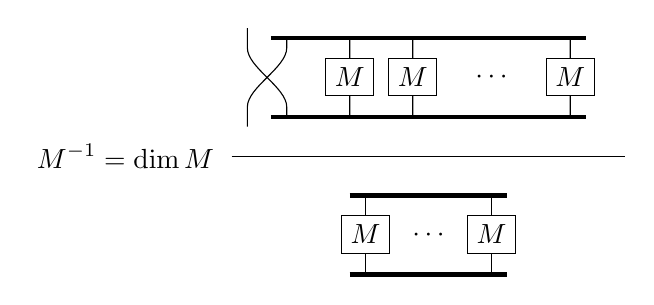
\begin{tikzpicture}%[scale=.8]
    \coordinate(O1)at(0,0);
    \coordinate(O2)at(0,-1);
    \coordinate(L)at(-.5,-1.5);
    \coordinate(D1)at(1,-2);
    \coordinate(D2)at(1,-3);
    \node at(-.6,-1.5)[anchor=east]{$\displaystyle M^{-1}=\dim M$};
    \draw[ultra thick]
        (O1)--++(4,0)
        (O2)--++(4,0)
    ;
    % adjugate matrix
    \draw
        (O1)++(1,0)--++(0,-.25)
        node[anchor=north, draw, rectangle](M1){$M$}
        (O2)++(1,0)--(M1.south)
        (O1)++(1.8,0)--++(0,-.25)
        node[anchor=north, draw, rectangle](M3){$M$}
        (O2)++(1.8,0)--(M3.south)
        (O1)++(3.8,0)--++(0,-.25)
        node[anchor=north, draw, rectangle](M2){$M$}
        (O2)++(3.8,0)--(M2.south)
        (O1)++(2.8,0)++(0,-.5)
        node[anchor=center]{$\cdots$}
        (O1)++(.2,0)--++(0,-.125)
        .. controls ++(0,-.25) and ++(0,.25) .. ++(-.5,-.75)
        --++(0,-.25)
        (O2)++(.2,0)--++(0,.125)
        .. controls ++(0,.25) and ++(0,-.25) .. ++(-.5,.75)
        --++(0,.25)
    ;
    \draw
        (L)--++(5,0)
    ;
    % determinant
    \draw[ultra thick]
        (D1)--++(2,0)
        (D2)--++(2,0)
    ;
    \draw
        (D1)++(.2,0)--++(0,-.25)
        node[anchor=north, draw, rectangle](B1){$M$}
        (D2)++(.2,0)--(B1.south)
        (D1)++(1.8,0)--++(0,-.25)
        node[anchor=north, draw, rectangle](B2){$M$}
        (D2)++(1.8,0)--(B2.south)
        (D1)++(1,0)++(0,-.5)
        node[anchor=center]{$\cdots$}
    ;
\end{tikzpicture}
